% Diagrama Geral do Sistema
\section{Diagrama Geral do Sistema}

\label{pro:dgs}

\begin{figure}[htp]
  \begin{center}
    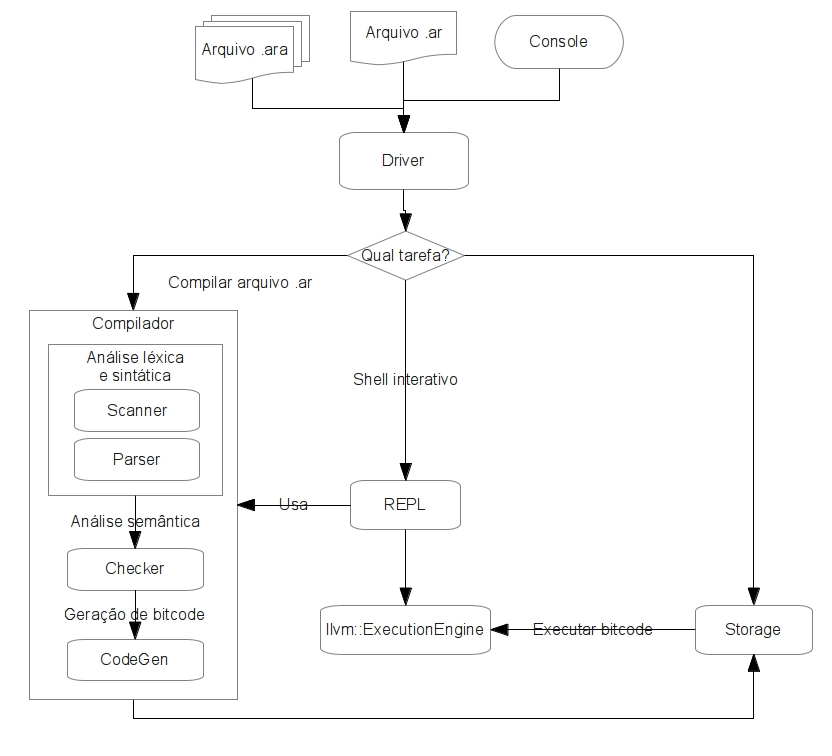
\includegraphics[width=1\textwidth]{figuras/dgs}
  \end{center}
  \caption{Diagrama Geral do Sistema}
  \label{fig:dgs}
\end{figure}

No diagrama podemos ver a estrutura interna b\ah sica do sistema proposto. Um arquivo \emph{.ar} \eh\ o arquivo que cont\eh m a linguagem fonte utilizada pelos processos de compila\ca o e interpreta\ca o por arquivo.

Um arquivo \emph{.ara} cont\eh m um conjunto de arquivos pr\eh-compilados no formato bin\ah rio \emph{bitcode}, armazenados em um arquivo \emph{.zip}, que ser\ao\ utilizados pela \emph{llvm::ExecutionEngine} executar as tarefas definidas no c\oh digo fonte original.

H\ah\ tamb\eh m o modelo \emph{REPL} que \eh\ ativado atrav\eh s do programa console\footnote{Console, prompt de comando ou terminal de comandos.} do sistema operacional, dispondo uma ferramenta de interpreta\ca o e execu\ca o de express\~o es para o usu\ah rio.

O objeto \emph{Driver} \eh\ respons\ah vel por entender e direcionar o trabalho do sistema.

O objeto \emph{Storage} \eh\ respons\ah vel por abstrair e controlar a manipula\ca o dos arquivos no sistema, que depende tamb\eh m de especificidades do sistema operacional hospedeiro.
